\documentclass[11pt]{article}
\usepackage[margin=1in]{geometry}
\usepackage{amsmath,amssymb,amsthm,mathtools}
\usepackage{graphicx}
\usepackage[hidelinks]{hyperref}
\usepackage{xcolor}

\newtheorem{theorem}{Theorem}
\newtheorem{lemma}[theorem]{Lemma}
\newcommand{\C}{\mathbb C}
\newcommand{\N}{\mathcal N}
\setlength{\emergencystretch}{2em}

\title{A $2$-partial isometry whose canonical generalized inverse\\
cannot be Moore--Penrose for any Hilbert inner product}
\author{Autonomous mathematical discovery run \texttt{fa\_banach\_001}}
\date{17 August 2026}

\begin{document}
\maketitle

\noindent\textbf{Status.}
Candidate full negative answer, likely valid pending expert review.

\section{Source question}

Aouichaoui, Bucha\l a, and Garcia observe that if $T$ is a
$2$-partial isometry, then
\[
 S=2T^*-T^{*2}T
\]
is a generalized inverse of $T$, with $ST$ an orthogonal projection for the
original inner product.  Their Question~6 asks whether this fixed operator
$S$ is the Moore--Penrose inverse of $T$ with respect to \emph{some} Hilbert
inner product on the same space \cite[Question~6, PDF p.~17]{ABG}.

\begin{center}
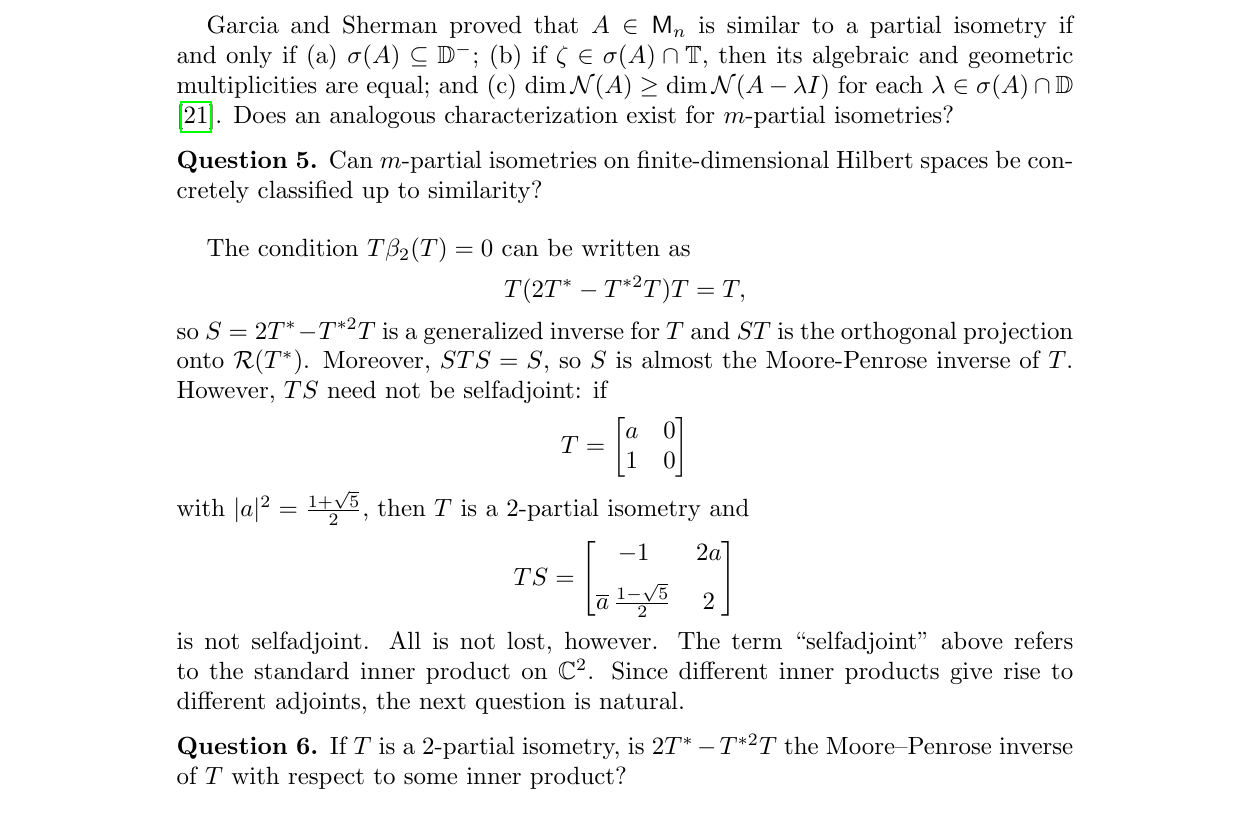
\includegraphics[width=0.84\textwidth]{figures/open_question.png}
\end{center}

We give a negative answer.  In fact, the $2\times2$ matrix displayed
immediately before the question in the source already supplies a
counterexample.

\section{Proof intuition}

Changing the inner product on $\C^2$ amounts to choosing a positive definite
Hermitian matrix $G$.  A fixed operator $A$ is selfadjoint for the new inner
product exactly when $A^*G=GA$.

For the source's example, the two idempotents in the Penrose equations are
\[
 ST=\begin{pmatrix}1&0\\0&0\end{pmatrix}
 \quad\text{and}\quad
 TS=\begin{pmatrix}-1&2a\\a\delta&2\end{pmatrix},
 \qquad \delta<0.
\]
Making $ST$ selfadjoint forces $G$ to be diagonal.  Making $TS$ selfadjoint
with respect to the same diagonal $G=\operatorname{diag}(x,y)$ would then
force $2x=\delta y$.  The left side is positive and the right side negative.
Thus no Hilbert inner product can make both Penrose idempotents selfadjoint.

\section{Counterexample}

We first record the standard change-of-inner-product test.

\begin{lemma}\label{lem:test}
Let $T,S\in M_n(\C)$ satisfy $TST=T$ and $STS=S$.  The operator $S$ is the
Moore--Penrose inverse of $T$ for the inner product
\[
 \langle x,y\rangle_G=\langle Gx,y\rangle,
 \qquad G=G^*>0,
\]
if and only if
\[
 (TS)^*G=G(TS)
 \quad\text{and}\quad
 (ST)^*G=G(ST).
\]
\end{lemma}

\begin{proof}
The adjoint for this inner product is $A^{\sharp}=G^{-1}A^*G$.  The first two
Penrose equations are already the two assumed generalized-inverse identities.
The remaining two say precisely that $TS$ and $ST$ are
$\sharp$-selfadjoint, which is equivalent to the displayed matrix equations.
\end{proof}

\begin{theorem}\label{thm:main}
Question~6 of \cite{ABG} has a negative answer.  More explicitly, let
\[
 \varphi=\frac{1+\sqrt5}{2},\qquad
 a=\sqrt\varphi,\qquad
 \delta=1-\varphi=\frac{1-\sqrt5}{2},
\]
and define
\[
 T=\begin{pmatrix}a&0\\1&0\end{pmatrix}.
\]
Then $T$ is a $2$-partial isometry, but
\[
 S=2T^*-T^{*2}T
\]
is not the Moore--Penrose inverse of $T$ with respect to any Hilbert inner
product on $\C^2$.
\end{theorem}

\begin{proof}
Since $a^2=\varphi$ and $\varphi^2=\varphi+1$, direct multiplication gives
\[
 T^*T=\begin{pmatrix}\varphi+1&0\\0&0\end{pmatrix},
 \qquad
 T^{*2}T^2=\begin{pmatrix}\varphi^2+\varphi&0\\0&0\end{pmatrix}.
\]
Consequently,
\[
 \beta_2(T)=T^{*2}T^2-2T^*T+I
 =\begin{pmatrix}
 \varphi^2-\varphi-1&0\\0&1
 \end{pmatrix}
 =\begin{pmatrix}0&0\\0&1\end{pmatrix}.
\]
Thus $T\beta_2(T)=0$, so $T$ is a $2$-partial isometry.

Using $2-\varphi^2=1-\varphi=\delta$, we obtain
\[
 S=\begin{pmatrix}a\delta&2\\0&0\end{pmatrix}.
\]
Because $\delta\varphi=-1$,
\begin{equation}\label{eq:PQ}
 P:=ST=\begin{pmatrix}1&0\\0&0\end{pmatrix},
 \qquad
 Q:=TS=\begin{pmatrix}-1&2a\\a\delta&2\end{pmatrix}.
\end{equation}
In particular, $TST=T$ and $STS=S$, so $S$ is indeed a generalized inverse.

Suppose, toward a contradiction, that $S$ were the Moore--Penrose inverse for
some Hilbert inner product.  Relative to the original coordinates, this
inner product is represented by a positive definite Hermitian matrix
\[
 G=\begin{pmatrix}x&z\\\overline z&y\end{pmatrix}.
\]
By Lemma~\ref{lem:test}, $P^*G=GP$.  Using the first matrix in
\eqref{eq:PQ}, this equality forces $z=0$.  Hence
$G=\operatorname{diag}(x,y)$ with $x,y>0$.

The $(1,2)$ entry of the remaining identity $Q^*G=GQ$ is
\[
 a\delta y=2ax,
\]
or, since $a>0$,
\[
 \delta y=2x.
\]
This is impossible: $x,y>0$ while $\delta<0$.  Therefore no positive
definite $G$ satisfies the two adjoint equations, and Lemma~\ref{lem:test}
proves the claim.
\end{proof}

\section{Scope, verification, and novelty}

The theorem fully answers the universal yes/no Question~6 negatively.  It
does not classify which $2$-partial isometries have a canonical generalized
inverse that becomes Moore--Penrose after renorming, nor does it address the
paper's broader Questions~1--5.

The accompanying exact-arithmetic script verifies $T\beta_2(T)=0$, the formula
for $S$, both generalized-inverse identities, and the two linear equations in
the entries of $G$.  The script is a regression check and is not needed for
the proof.

A bounded novelty search on 17 August 2026 covered the four run indexes, the
current arXiv record (still version~1), exact searches for the title and
Question~6, and variants combining $2$-partial isometries, Moore--Penrose
inverses, and changes of inner product.  No later answer was found.  Because
the source appeared only in June 2026, novelty confidence is moderate pending
specialist review.

\paragraph{Human review recommendation.}
Check the interpretation that the displayed $S=2T^*-T^{*2}T$ is fixed while
the inner product is varied, as the wording of Question~6 indicates.  Then
check the four products in \eqref{eq:PQ} and the two $G$-selfadjointness
equations; no external structural theorem is used.

\begin{thebibliography}{9}
\raggedright
\bibitem{ABG}
M. A. Aouichaoui, M. Bucha\l a, and S. R. Garcia,
\emph{On $m$-partial isometries: spectra, weighted shifts, and similarity},
arXiv:2606.12865v1 (2026).
\end{thebibliography}

\end{document}
